\documentclass{eecslides}
\usepackage{amsmath}
\usepackage{color}
\usepackage{listings}
\usepackage{multimedia}
\definecolor{lgray}{gray}{0.9}
\lstset{ %
language=R,                		% choose the language of the code
basicstyle=\tiny,       % the size of the fonts that are used for the code
numbers=left,                  	% where to put the line-numbers
numberstyle=\footnotesize,   % the size of the fonts that are used for the line-numbers
stepnumber=1,                   	% the step between two line-numbers. If it is 1 each line will be numbered
numbersep=5pt,                  	% how far the line-numbers are from the code
backgroundcolor=\color{lgray},  % choose the background color. You must add \usepackage{color}
showspaces=false,              	% show spaces adding particular underscores
showstringspaces=false,         % underline spaces within strings
showtabs=false,                 	% show tabs within strings adding particular underscores
frame=single,           		% adds a frame around the code
tabsize=2,          			% sets default tabsize to 2 spaces
captionpos=b,           		% sets the caption-position to bottom
breaklines=true,        		% sets automatic line breaking
breakatwhitespace=false,    	% sets if automatic breaks should only happen at whitespace
escapeinside={\%*}{*)}          	% if you want to add a comment within your code
}
\setbeamertemplate{enumerate items}[default]
%------------------------------

\title[Spatial models]{Spatial models in ecology}
\subtitle{Analytical and numerical methods}
\author[D. Gravel]{Dominique Gravel}
\institute[Chaire de recherche EEC]{UQAR -- Chaire de Recherche EEC}
\website{http://www.chaire-eec.uqar.ca/}
\date{\today}

\begin{document}

	\begin{frame}[plain]
		\titlepage
	\end{frame}

	\begin{frame}[plain]{Outline}
		\tableofcontents
	\end{frame}

%------------------------------
%------------------------------
	\section{Introduction}
%------------------------------
%------------------------------

	\begin{frame}{Exercise}

	Program a random walk model. Consider a single individual whose spatial coordinates at time $t_0$ are $(0,0)$. Now consider the following simple rule: each time step, pick up randomly $(X,Y)$ coordinates among the eight immediate neighbours with a single unit movement in direction $X$ and $Y$ with probability $0.5$.

	\begin{itemize}
		\item Plot the spreading of the individual over time
		\item Run the model 100 times and record the distance of the individual at time t = 10 and t = 100
	\end{itemize}

	\end{frame}

%------------------------------

	\begin{frame}{Exercise}{Brownian motion}

	\textbf{Definition:} random moving of particles suspended in a fluid (a liquid or a gas) resulting from their bombardment by the fast-moving atoms or molecules in the gas or liquid.
	\vskip 1em

	Could be use to detect non random features of random number generators.
	\vskip 1em

	An old and rich litterature on diffusion equations and its connection to random walk process. Connecting diffusion and Brownan motion was one of Einstein's three accomplishments that earned hum his Nobel prize!
	\vskip 1em

	In ecology, it forms the basis of a class of spatial models. More generally it is fundamental to understand spatial spreading, of organisms and disturbances. Random walk is the driving force beind neutral models. Also used to study the structure of phylogenetic trees. 

	\end{frame}

%------------------------------

	\begin{frame}{Important spatial processes in ecology}

		\begin{columns}
			\begin{column}{0.5\textwidth}
			\begin{itemize}
				\item Dispersal
				\item Natural disturbances
				\item Synchrony, Moran effect
				\item Spreading of invasive species
				\item Metapopulation dynamics, fragmentation, habitat loss
				\item Species distribution
				\item Estimating species diversity
			\end{itemize}	
			\end{column}
%----
			\begin{column}{0.5\textwidth}
				\begin{center}
					\includegraphics[height=0.3\textheight]{fragmentation}
				\end{center}
				\begin{center}
					\includegraphics[height=0.3\textheight]{range}
				\end{center}
			\end{column}
		\end{columns}	 


	\end{frame}

%------------------------------

	\begin{frame}{The importance of spatial structure}

		\begin{columns}
			\begin{column}{0.4\textwidth}
			\begin{itemize}
				\item Why?
				\item What characteristics? (e.g. stationarity, dynamics, scale etc...)
				\item Impacts?
			\end{itemize}	
			\end{column}
%----
			\begin{column}{0.6\textwidth}
				\begin{center}
					\includegraphics[height=0.7\textheight]{rietkerk}
				\end{center}
			\end{column}
		\end{columns}	 

	\end{frame}

%------------------------------

	\begin{frame}{Distinguishing types of spatial models}
		\begin{itemize}
			\item Space 
			\item Time
			\item State variable
		\end{itemize}	
	\end{frame}

%------------------------------

	\begin{frame}{Distinguishing types of spatial models}
	
	Discrete space\\	
		\begin{itemize}
			\item Patch models (2, 3,...,n)
			\item Landscape models
			\item Cellular automaton
			\item Lattice models
		\end{itemize}
	\vskip 1em

	Continuous space\\	
		\begin{itemize}
			\item Microscopic models 
			\item Macroscopic models
		\end{itemize}
	\end{frame}

%------------------------------
%------------------------------
	\section{Objectives}
%------------------------------
%------------------------------

	\begin{frame}{Conceptual objectives}
		\begin{itemize}
			\item Diffusion process
			\item Cellular automaton
			\item Metapopulation dynamics \& spatially explicit dispersal
		\end{itemize}
	\end{frame}

%------------------------------

	\begin{frame}{Technical objectives}
		\begin{itemize}
			\item Partial differential equations
			\item Cellular automaton
			\item Analysis of spatial structure (patch size distribution)
			\item Introduction to root solving
			\item Program spatially explicit dispersal
		\end{itemize}
	\end{frame}

%------------------------------
%------------------------------
	\section{Diffusion}
%------------------------------
%------------------------------

	\begin{frame}{Diffusion model}{Analytical solution}

	In this section, we will derive a model expressing the change in density (dynamics) continuously over space, time and the state variable. First, consider a dispersal kernel $K(y,x)$ giving the probability that an individidual leaving position $y$ ends up at position $x$.\\
	\vskip 1em

	Now suppose that individuals leaves location $x$ at rate $\phi$. This movement means that the number lof loss individuals from any particular location $x$ is $\phi n(x,t)$. 
	\vskip 1em
	
	\end{frame}

%------------------------------

	\begin{frame}{Diffusion model}{Analytical solution}
	And similarly, the number of individuals going from location $y$ to location $x$ is $\phi n(y,t)K(y,x)$. Note that because all individuals must land somewhere, the integral $\int K(y,x)dy$ must be equal to 1. The movement for a one dimensional system can therefore be described as follow:\\
	$\frac{\partial n(x,t)}{\partial t} = \phi \int K(y,x)n(y,t)dy - \phi n(x,t)$
	\vskip 1em

	The left hand side of the equation represents the immigration, while the right hand side represents emigration. This equation is named \emph{integrodifferential} and it has been shown that we could recover the diffusion equation from it. 
	\end{frame}

%------------------------------
%------------------------------

	\begin{frame}{Diffusion model}{Analytical solution}
		We begin with a Taylor series expansion of $n(y,t)$ about position $x$:\\
		$n(y,t) = n(x,t) + \frac{\partial n(x,t)}{\partial x}(y-x) + \frac{1}{2}\frac{\partial^2n(x,t)}{\partial x^2}(y-x)^2+....$
		\vskip 1em

		And throw in equation (9.1) to get the ugliest equation ever:\\
		$\frac{\partial n(x,t)}{\partial t} = \phi \int K(y,x)[n(x,t) + \frac{\partial n(x,t)}{\partial x}(y-x) + \frac{1}{2}\frac{\partial^2n(x,t)}{\partial x^2}(y-x)^2]dy - \phi n(x,t)$
		\vskip 1em

		 I will skip the simplifications, but just keep in mind that if movement is symetric (there is no bias toward one direction) and we respect the condition of the dispersal kernel having an integral equal to 1, then by some magical trick we obtain the nice equation (trust me, or at least Wilson 2000!):\\	
		$\frac{\partial n(x,t)}{\partial t} = D\frac{\partial^2 n}{\partial x^2}$
		\vskip 1em
		
		Isn't it convenient? Parameter $D = \phi R^2/2$ is the diffusion coefficient, and $R$ is the mean square displacement distance.
		\end{frame} 

%------------------------------

	\begin{frame}{Diffusion model}{Analytical solution}

		Diffusion tends to homogenize the distribution of organisms and therefore one solution to the diffusion equation is a constant uniform distribution, $n(x,t) = n*$. This result is somewhat trivial, and therefore a more interesting question is \emph{What are the temporal dynamics of a small spatial perturbation about this equilibrium solution?}
		\vskip 1em

		Formalizing the problem of spatial stability, we assume a spatiotemporal perturbation described by the function\\
		$n(x,t) = n* + n_0e^{-t/T}sin\frac{2\pi x}{L}$
		\vskip 1em

		where $n_0$ represents the initial perturbation at time $t = 0$. The first factor $e^{-t/T}$ is a time-dependent decay function, which multiplies the amplitiude by $1/e$ when $t = T$. The factor $sin\frac{2\pi x}{L}$ represents the spatial variation of the intitial perturbation. Parameterl $L$ is the perturbation's wavelength and represent peak to peak distance. 
	\end{frame}

%------------------------------

	\begin{frame}{Diffusion model}{Analytical solution}
		We now conduct a stability analyslis by substituing the latest equation for the perturbation in the diffusion model:\\
		$\frac{\partial}{\partial t} (n* + n_0e^{-t/T}sin\frac{2\pi x}{L}) = D\frac{\partial^2}{\partial x^2}(n* + n_0e^{-t/T}sin\frac{2\pi x}{L})$\\
		\vskip 1em
		
		We are again stuck with an unreadable equation (unfortunately this is systematically the case with spatial models....). But after some algebra found in a good text book, we obtain the simplified solution:\\
		$ T = \frac{L^2}{4\pi^2D}$
		\vskip 1em

		which is not much meaningful in first sight. It basically tells us that the time for a perturbation of a given structure $L$ to dissipate is inversely proportional to diffusion rate $D$.  

	\end{frame}

%------------------------------

	\begin{frame}{Diffusion model}{Analytical solution}
	A more interesting case arises when we add \emph{reaction}, i.-e. a local interaction among organisms (in other words, when we add ecology!). 
	\vskip 1em

	The simplest diffusion-reaction model was originally studied by Fisher and later by Skellam. In one dimension, the density changes according to the following equation:\\
	$\frac{\partial N}{\partial t} =D \frac{\partial^2 N}{\partial x^2} + rN$\\
	\vskip 1em

	with boundary conditions:\\
	$N(x = 0, t = 0) = N_0$\\
	$N(x = \pm \infty, t)$ is finite
	\vskip 1em

	Skipping the tedious integration of the model, we get the solution:\\
	$N(x,t) = \frac{N_0}{2\sqrt{\pi Dt}}e^{kt-\frac{x^2}{4Dt}}$
	\end{frame}

%------------------------------

	\begin{frame}{Ploting the result}

		\begin{center}
			\includegraphics[height=0.8\textheight]{fig5_4}
		\end{center}

	\end{frame}

%------------------------------

	\begin{frame}{Diffusion model}{Analytical solution}

		The most meaningful result comes from the study of spreading rate of invading organisms. Following Kellam's (1953) derivations of the Fisher's diffusion model with logistic growth, we obtain the following spreading rate:\\
		$ S =2\sqrt{rD}$
		\vskip 1em

		which holds with standard diffusion or an exponential dispersal kernel. This equation basically tells us three things:
		\begin{itemize}
			\item Spreading increases with the square root of the diffusion coefficient (which happens to be the square of the mean dispersal distance - trivial result)
			\item It also increases with the growth rate in the invading area
			\item Carrying capacity in the resident area does not impact migration rate (note that it might under other model formulations) 
		\end{itemize}

	\end{frame}

%------------------------------

	\begin{frame}{Diffusion model}{Numerical integration}

	Numerical integration in time: jumping from one point in time to the next. 
	\vskip 1em

	Numerical integration in space: computation of the fvalue of the function in a finite number of discriete spatial locations. 
	\vskip 1em 

	Consider the Kolmogorov diffusion equation on a one dimension landscape:\\
	$\frac{\partial N}{\partial t} = - \frac{\partial Flux}{\partial x} + rN(1-\frac{N}{K})$
	\vskip 1em

	where\\
	$\frac{\partial Flux}{\partial x} = D \frac{\partial N}{\partial x}$\\

	\end{frame}

%------------------------------

	\begin{frame}{Diffusion model}{Numerical integration}

	We numerically approximate the rate of change in one cell $i$ as (be aware of the switch to ODEs): \\
	$\frac{dN_i}{dt} = - \frac{\Delta_i Flux}{\Delta x_i} + + rN_i(1-\frac{N_i}{K})$\\
	$\frac{dN_i}{dt} = - \frac{Flux_{i,i+1}}{Flux_{i-1,i}} + + rN_i(1-\frac{N_i}{K})$
	\vskip 1em

	where $\Delta x_i$ is the length of the cell and $\Delta_i$ denotes that the flux gradient is to be taken around the cell $i$. In other words, as the difference of the flues at the interfacte with the next cell $(i,i+1)$ and the previous one, $(i-1,i)$. 
	\vskip 1em

	The flux is simply given by:\\
	$Flux_{i-1,i} = -D_{i-1,i}\frac{N_i-N_{i-1}}{\Delta x_{i-1,i}}$
	\vskip 1em

	where $\Delta x{i-1,i}$ is the dispersion distance, ie the distance between adjacent cells. 

	\end{frame}

%------------------------------

	\begin{frame}[fragile]{Implementation in R}{Parameters}
	
		\begin{lstlisting}
			# Diffusion rate (m2/time)
			D = 0.3    
			
			# Intrinsic growth rate
			r = 0.05   

			# Carrying capacity
			K = 1

			# Cell size
			delx = 1

			# Number of cells
			numboxes = 60 
	
			# Sequence
			Distance = seq(from=0.5,by=delx,length.out=numboxes)
		\end{lstlisting}

	\end{frame}

%------------------------------
	
	\begin{frame}[fragile]{Implementation in R}{The model equations}
	
	We use here the diffusion-reaction equation discretized per cell to calculate the rate of change in each cell. There are therefore \emph{numboxes} differential equations. The flux between cells is calculated using the function \emph{diff}, which takes the gradient between adjacent locations.\\
		\begin{lstlisting}
			model <-function(t,N,parameters)
				{
				deltax     <- c (0.5,rep(1,numboxes-1),0.5)    
				Flux       <- -D*diff(c(0,N,0))/deltax
				dN    <- -diff(Flux)/delx  + r*N*(1-N/K)

				# the output: the rate of change in each cell
				list(dN)
			}  # end of model
		\end{lstlisting}

	\end{frame}

%------------------------------
	
	\begin{frame}[fragile]{Implementation in R}{Initial conditions}
	
	Densities are initiated with 0 in all cells, except for the two central ones, which are at carrying capacity.\\
		\begin{lstlisting}
			N = rep(0,times=numboxes)       # individuals/surface

			N[30:31] = K

			state = c(N=N)            # the state variables are initialised

		\end{lstlisting}

	\end{frame}

%------------------------------
	
	\begin{frame}[fragile]{Implementation in R}{Running the model}
	
	The model is simply run using the function \emph{ode} of the package \emph{deSolve}.\\
		\begin{lstlisting}
		
			times = seq(0,200,by=1)   # output wanted at these time intervals           

			out = ode(state,times,model,parms=0)  # ode is integration routine

			DENSITY   <- out[,2:(numboxes  +1)]

		\end{lstlisting}

	\end{frame}

%------------------------------
	
	\begin{frame}[fragile]{Implementation in R}{Ploting the resultsl}
	
	Here I use directly the code provided in Soetaert's book (as a did for a big chunk of the slides...).\\
		\begin{lstlisting}
		
			# set margins
			par(mfrow=c(1,1))
			par(oma=c(0,0,3,0))   

			# set colors
			color= topo.colors

			# make the plot
			filled.contour(x=times,y=Distance,DENSITY,color= color,
			xlab="time", ylab= "Distance",main="Density")

		\end{lstlisting}

	\end{frame}

%------------------------------
	
	\begin{frame}[fragile]{Implementation in R}{Ploting the results}

		\begin{figure}[!t]
			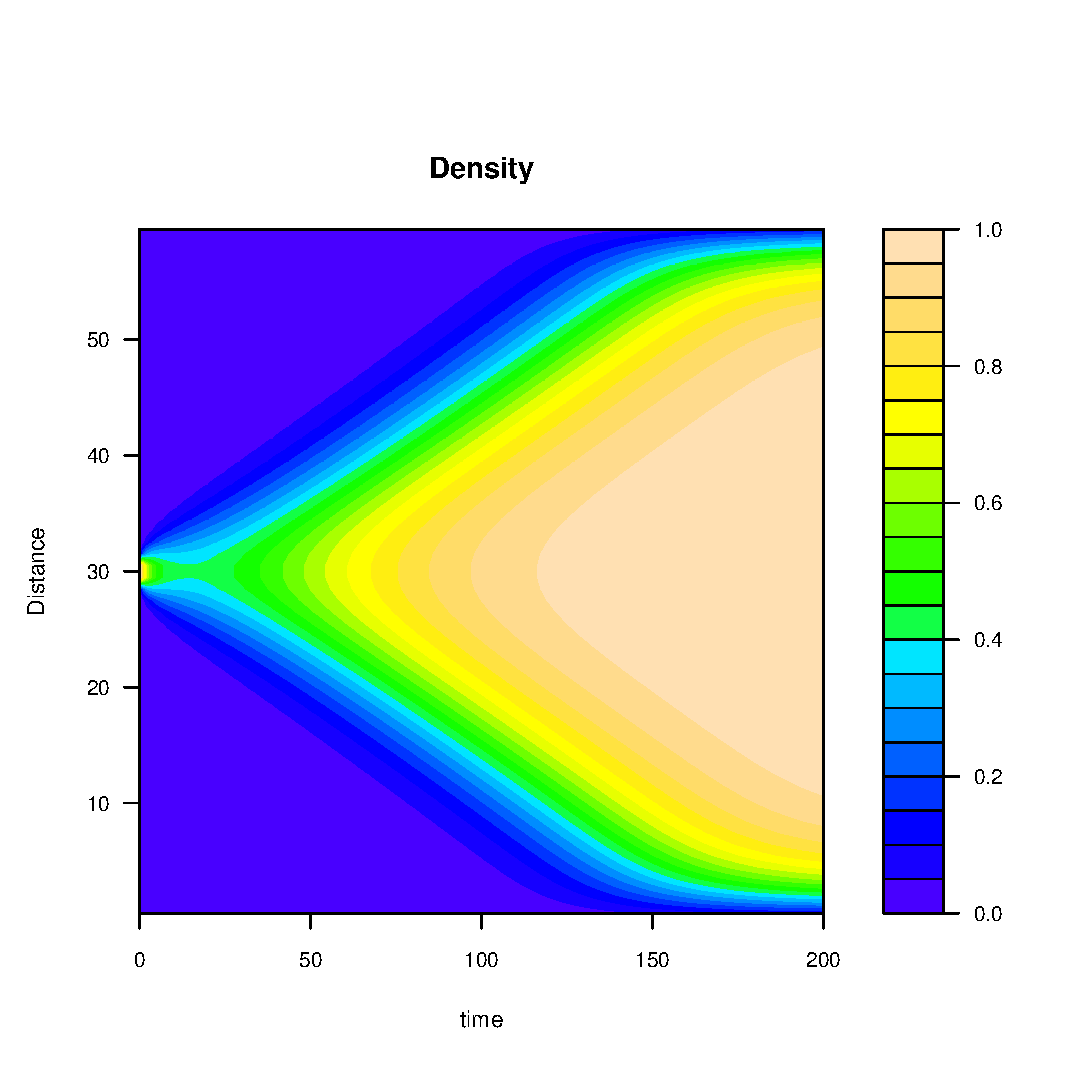
\includegraphics[height=0.75\textheight]{diffusion_reaction}
		\end{figure}

	\end{frame}

%------------------------------
	
	\begin{frame}[fragile]{Diffusion and pretty patterns}{Turing instabilities}

		\begin{figure}[!t]
			\includegraphics[height=0.75\textheight]{rietkerk2}
		\end{figure}

	\end{frame}

%------------------------------
	
	\begin{frame}{Exercise}

		Now program a diffusion version of the Rosensweig-MacArthur model of predator-prey interactions. You should eventually get to a result similar to what Jansen (2000) found:\\

		\begin{figure}[!t]
			\includegraphics[height=0.55\textheight]{Jansen2000}
		\end{figure}

	\end{frame}


%------------------------------
%------------------------------
	\section{Cellular automaton}
%------------------------------
%------------------------------

	\begin{frame}{Cellular automaton}{Definition}

	\begin{itemize}
		\item Discrete space. Divided in cells, culd be 1D, 2D or 3D
		\item Cells could be in different \emph{states}
		\item Cell state changes in discrete time
		\item All cells could be updated at once, or subsequently	
		\item Changes obey rules, which could be deterministic or stochastic
		\item Transition rules are function of the state of the focal cell and the neighbours
	\end{itemize}
	\end{frame}

%------------------------------

	\begin{frame}{Cellular automaton}{History}
	
	\textbf{Fundamental question:} is it possible to generate complex and non random structures from simple rules?

		\begin{itemize}
			\item Computer science, maths \& physics
			\item Von Nuemann (~1940)
			\item Conway (~1970)
			\item Wolfram (~1980)
		\end{itemize}
	\end{frame}

%------------------------------
	\begin{frame}{Landscape structure}

		\begin{figure}[!t]
			\includegraphics[height=0.35\textheight]{landscape_types}
		\end{figure}

	\end{frame}

%------------------------------

	\begin{frame}{States}

		\begin{figure}[!t]
			\includegraphics[height=0.55\textheight]{states}
		\end{figure}

	\end{frame}

%------------------------------

	\begin{frame}{Neighborhood types}

		\begin{figure}[!t]
			\includegraphics[height=0.35\textheight]{neighbourhood}
		\end{figure}

	\end{frame}

%------------------------------

	\begin{frame}{Neighborhood types}

		\begin{figure}[!t]
			\includegraphics[height=0.35\textheight]{high_neighbourhood}
		\end{figure}

	\end{frame}

%------------------------------

	\begin{frame}{Transitions}

		\begin{figure}[!t]
			\includegraphics[height=0.55\textheight]{transitions}
		\end{figure}

	\end{frame}

%------------------------------

	\begin{frame}{Boundary conditions}{Buffer zone}

		\begin{figure}[!t]
			\includegraphics[height=0.55\textheight]{buffer}
		\end{figure}

	\end{frame}

%------------------------------

	\begin{frame}{Boundary conditions}{Mirror}

		\begin{figure}[!t]
			\includegraphics[height=0.55\textheight]{mirror}
		\end{figure}

	\end{frame}

%------------------------------

	\begin{frame}{Boundary conditions}{Torus}

		\begin{figure}[!t]
			\includegraphics[height=0.55\textheight]{torus}
		\end{figure}

	\end{frame}

%------------------------------

	\begin{frame}{Transitions}

		\begin{figure}[!t]
			\includegraphics[height=0.55\textheight]{transitions}
		\end{figure}

	\end{frame}

%------------------------------

	\begin{frame}{Example}{Wolfram's rules}

	Simple deterministic rules (possibility of 256) to determine the transition between white (0) and black (1) cells. 
	\vskip 1em

	A classic example: rule 90
	\begin{itemize}
		\item Adding two white cells gives a white cell
		\item Adding to black cells gives a white cell
		\item Adding one white and one black gives a black
	\end{itemize}

	\end{frame}

%------------------------------

	\begin{frame}[fragile]{Example}{package CellularAutomaton}

		\begin{lstlisting}
			library(CellularAutomaton)
		
			# Example with rule 90 and run for 100 time steps
			res = CellularAutomaton(n = 90, t = 100) 
			res$plot()
	
		\end{lstlisting}

		\begin{figure}
			\includegraphics[height=0.55\textheight]{rule90}
		\end{figure}

	\end{frame}

%------------------------------

	\begin{frame}{Rule 90 in nature!}

		\begin{figure}[!t]
			\includegraphics[height=0.55\textheight]{snail}
		\end{figure}

	\end{frame}

%------------------------------

	\begin{frame}{Wolfram's classification}

		\begin{columns}
			\begin{column}{0.5\textwidth}
				\begin{itemize}
					\item Stable \& homogeneous
					\item Periodic
					\item Chaotic or aperiodic
					\item Complex
				\end{itemize}
			\end{column}
%----
			\begin{column}{0.5\textwidth}
				\begin{center}
					\includegraphics[height=0.6\textheight]{ca_types}
				\end{center}
			\end{column}
		\end{columns}	 

	\end{frame}

%------------------------------

	\begin{frame}{Forest fire model}

		\begin{columns}
			\begin{column}{0.5\textwidth}
				Power law distribution of forest fire size
			\end{column}
%----
			\begin{column}{0.5\textwidth}
				\begin{center}
					\includegraphics[height=0.7\textheight]{power_law}
				\end{center}
			\end{column}
		\end{columns}	 
	\end{frame}

%%------------------------------

	\begin{frame}{Forest fire model}
		\begin{columns}
			\begin{column}{0.4\textwidth}
				\begin{itemize}
					\item CFS database
					\item All fires $>$ 200ha between 1960 and 1999
					\item Data for the Canadian Shield
				\end{itemize}
			\end{column}
%----
			\begin{column}{0.6\textwidth}
				\begin{center}
					\includegraphics[height=0.6\textheight]{fire}
				\end{center}
			\end{column}
		\end{columns}	 
	\end{frame}

%%------------------------------

	\begin{frame}{Forest fire model}
		
		What is the simplest model that could reproduce this structure?

	\end{frame}

%%------------------------------

	\begin{frame}{Forest fire model}{States}
		
	First model was published by the physicists Drossel \& Schabl (1992). Malamud et al. (1998) later published a simplification.

	Three possible states: 
		\begin{itemize}
			\item Empty
			\item Occupied by a three
			\item In fire
		\end{itemize}
	\end{frame}

%------------------------------

	\begin{frame}{Forest fire model}{Transition rules}

		\begin{itemize}
			\item A cell in fire turns into empty state
			\item An empty cell is colonized by a tree at probability $p$
			\item A cell occupied by a tree burns if one of the neighbours is in fire or burn at probability $f$ if no neighbour is in fire
		\end{itemize}
	\end{frame}

%%------------------------------

	\begin{frame}{Forest fire model}{Power law}
		\begin{center}
			\includegraphics[height=0.7\textheight]{fire_size}
		\end{center}
	\end{frame}

%------------------------------
%------------------------------
	\section{Dispersal}
%------------------------------
%------------------------------

	\begin{frame}{The metapopulation framework}{Levins model}

	Consider an ensemble of patches that could be either empty or occupied. Define $p$ as the fraction of the landscape that is occupied. The following model describes temporal dynamics of occupancy:\\
	$\frac{dp}{dt} = cp(1-p)-ep$
	\vskip 1em	

	where $c$ is the colonization rate and $e$ is the extinction rate. Solving the model at equilibrium yields:\\
	$p* = 1- \frac{e}{c}$
	\vskip 1em

	The fundamental result of metapopulation theory is that the species will persist provided that $c>e$.

	\end{frame}

%------------------------------

	\begin{frame}{The metapopulation framework}{Spatially explicit incidence function}

	The equilibrium occupancy will depend on the spatial distribution of the different patches. 

		\begin{columns}
			\begin{column}{0.5\textwidth}
				\begin{center}
					\includegraphics[height=0.4\textheight]{archipelago}
				\end{center}
	
			\end{column}
%----
			\begin{column}{0.5\textwidth}
				\begin{center}
					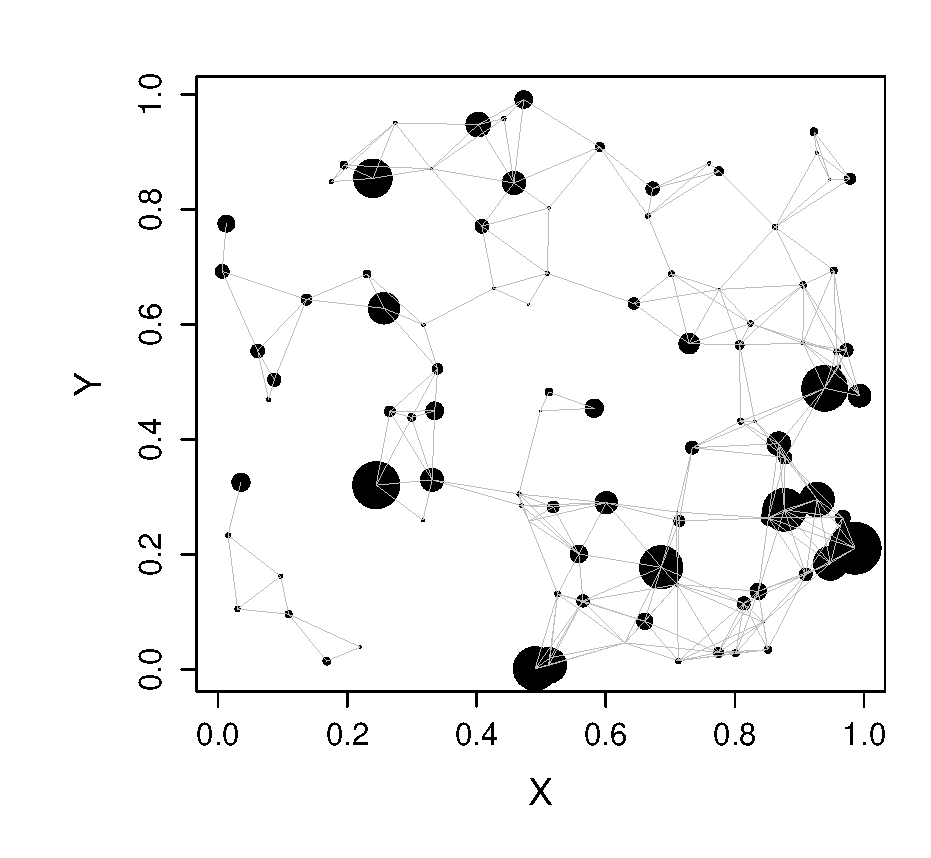
\includegraphics[height=0.5\textheight]{spatial_network}
				\end{center}
			\end{column}
		\end{columns}	 

	\end{frame}

%------------------------------

	\begin{frame}{The metapopulation framework}{Spatially explicit incidence function}

	Probability of an offspring leaving patch $y$m reaching patch $x$ and establishing a population is:\\
	$ c_yp_yk(y,x)A_y^b$
	\vskip 1em
	
	where $c_y$ is the number of offspring produced per unit of surface at patch $y$, $(y,x)$ is the dispersal kernel yielding the probability a single offspring leaving $y$ and getting to $x$, $p_y$ is the probability that patch $y$ is occupied, $A_y$ is the area of the patch $y$ and $b$ is a parameter relating area to the number of offspring produced. \\
	\vskip 1em

	Flipped around, the probability of that offspring not reaching that patch:\\
	$ 1 - c_yp_yk(y,x)A_y^b$
	\vskip 1em

	Considering all patches, we get the probability $C_x$ of at least one offspring reaching patch $x$ and establishing a population :\\
	$ 1 - \prod(1-c_yp_yk(y,x)A_y^b)$
	\vskip 1em

	\end{frame}
%------------------------------

	\begin{frame}{The metapopulation framework}{Spatially explicit incidence function}

	Looking at the other side of the equation, we have the extinction function:\\
	$E_i = \frac{e_x}{A_x^c}p_x$	
	\vskip 1em

	We now get the model:\\
	$\frac{dp_x}{dt} = C_x(1-p_x) - E_x$
	\vskip 1em

	And the equilibrium probability of occurrence at patch $x$:\\
	$p^x* = \frac{C_x}{C_x+E_x}$
	\vskip 1em

	This solution is a likelihood function that could be fitted to empirical data and used to evaluate the different parameters. 	We take the sum ($\sum p_x$) over all patches of the landscape to have the number of patches that are occupied:\\
	
	\end{frame}
%------------------------------

	\begin{frame}[fragile]{Solving the model on R}
		\begin{lstlisting}
			rm(list = ls())
			library(rootSolve)

			# Create a random metapop structure
			n = 100
			r = 0.15
			XY = cbind(runif(n), runif(n))
			A = rexp(n = n, rate = 1)

			distMat = as.matrix(dist(XY, method = 'euclidean', upper = T, diag = T))
			adjMat = matrix(0, nr = n, nc = n)
			adjMat[distMat < r] = 1
			diag(adjMat) = 0
		\end{lstlisting}
	\end{frame}
	
%------------------------------

	\begin{frame}[fragile]{Solving the model on R}
		\begin{lstlisting}
		# Plot the random landscape
		x11(height = 5.5, width = 6)
		par(mar=c(5,6,2,1))
		plot(XY[,1],XY[,2],xlab = "X", ylab = "Y",cex.lab = 1.5, cex.axis = 1.25,cex = A, pch = 19)
		adjVec = stack(as.data.frame(adjMat))[,1]
		XX = expand.grid(XY[,1],XY[,1])
		YY = expand.grid(XY[,2],XY[,2])
		XX = subset(XX,adjVec==1)
		YY = subset(YY,adjVec==1)
		arrows(x0 = XX[,1],x1=XX[,2],y0 = YY[,1], y1 = YY[,2], length = 0,lwd = 0.1, col = "grey")
		\end{lstlisting}
	\end{frame}
	
%------------------------------

	\begin{frame}{Solving the model on R}
		\begin{center}
			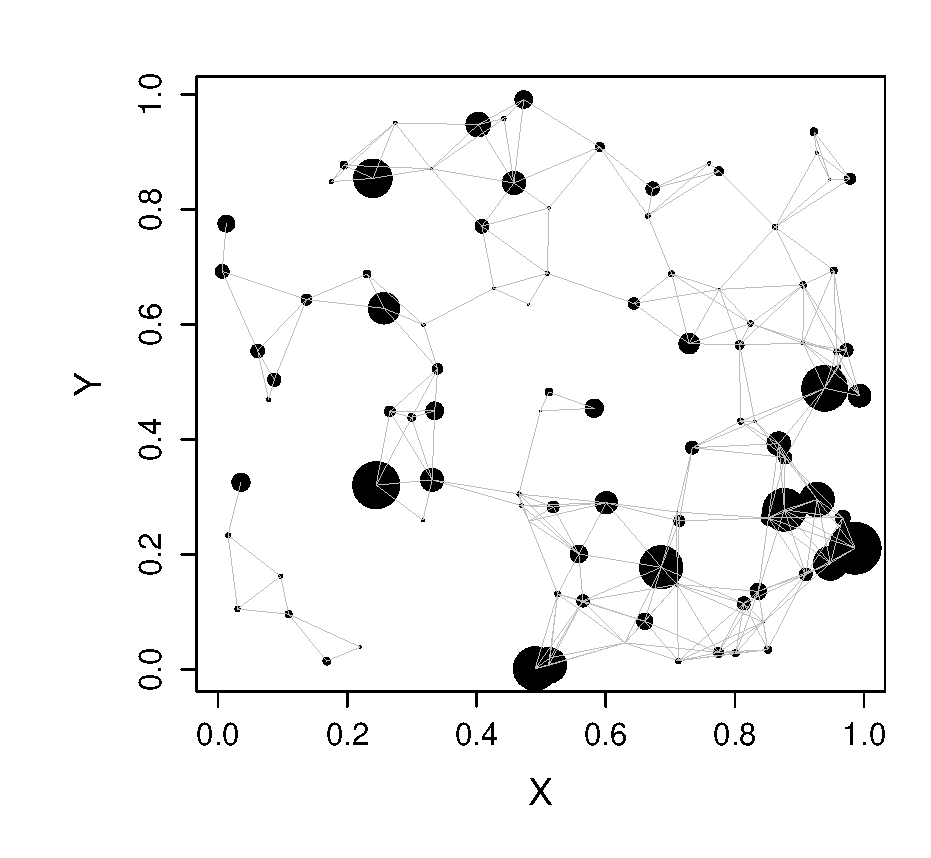
\includegraphics[height=0.7\textheight]{spatial_network}
		\end{center}
	\end{frame}
	
%------------------------------

	\begin{frame}[fragile]{Solving the model on R}
		\begin{lstlisting}
		# MAIN FUNCTION: 
		model1 = function(p,adjMat,A,b,c,e,f) {
			# Number of links per node
			degree = apply(adjMat,2,sum)

			# Weighted connectivity matrix
			adjMatw = adjMat*matrix(degree^-1,nr = n,nc=n, byrow=F) 
			adjMatw[adjMatw=="NaN"] = 0

			# Outgoing propagules
			emigr = f*A^b*p 

			# Pairwise colonization probability
			ColProbMat = adjMatw*matrix(emigr,nr = n,nc=n, byrow=F) 

			# Pairwise probability of no colonization even
			noColProbMat = 1 - ColProbMat	

			# Cumulative probability of an immigration event taking place
			ColProbVec = 1 - apply(noColProbMat,2,prod) 

			# Expected occupancy
			px = ColProbVec/(ColProbVec + e/A^c) - p
			return(px)
		}
		\end{lstlisting}
	\end{frame}
	
%------------------------------

	\begin{frame}[fragile]{Solving the model on R}
		\begin{lstlisting}
		# OPTIMIZATION
		get_px = function(adjMat,A,b,c,e,f) {
			degree = apply(adjMat,2,sum)
			model2 = function(p) model1(p,adjMat,A,b,c,e,f)
			
			# Start with the solution of a mean-field metapop model
			Start = numeric(n) + 1 - e/(mean(degree)*mean(A)^(b+c)*f) 

			# Perform the root solving
			multiroot(model2,start = Start,positive=TRUE)[[1]]
		}
		\end{lstlisting}
	\end{frame}
	
%------------------------------

	\begin{frame}[fragile]{Solving the model on R}
		\begin{lstlisting}
		# PLOTTING THE RESULTS
		# Solve the model
		eq_px = get_px(adjMat,A,b=0,c=0,e=0.1,f=0.5)

		# Rank the patches according to equilibrium occurrence probability
		RK = rank(eq_px)
		col = heat.colors(n = n)
		vec.col = numeric(n)
		for(i in 1:n) vec.col[i] = col[RK[i]]

		# Add points to the figure
		points(XY[,1],XY[,2],pch=21,bg=vec.col,cex = A)
		\end{lstlisting}
	\end{frame}
	
%------------------------------

	\begin{frame}{Solving the model on R}
		\begin{center}
			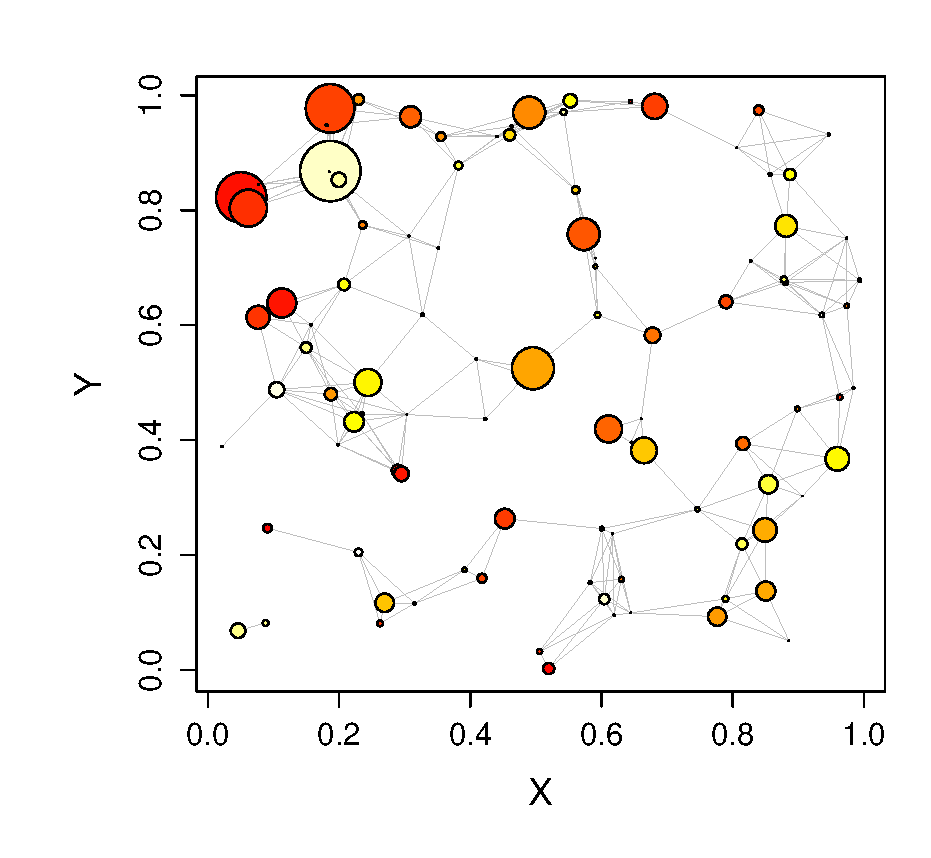
\includegraphics[height=0.7\textheight]{eq_metapop}
		\end{center}
	\end{frame}
	
%------------------------------

	\begin{frame}{Multi-species simulation model}
		See the following files:\\
		\begin{itemize}
			\item patch\_model
			\item lottery\_model
			\item examples
			\item spatial\_graphs
			\item simulations
		\end{itemize}
	\end{frame}
	
%------------------------------

%------------------------------
%------------------------------
\end{document}